%RLC_Circuits_P2
\chapter{Inductance and Series RLC circuits Part 2}
In our last lab, we used an oscilloscope to measure voltage and to plot it
as a function of time. Of course our Arduino can do this. You have seen the serial plotter already as you have used the Arduino software. But you may see a problem with building an actual oscilloscope. For one thing, our
signal generator voltage goes negative. Let's consider how we could design a circuit for our Arduino that will allow us to make this kind of measurement.

\section{The Instrument}

We have a new challenge. Our signal from our LRC circuit is sometimes negative. We will have truly negative voltages compared to our ground. Can we send a negative voltage into our Arduino? The answer is an emphatic NO! Negative voltages will also destroy our Arduino. But we really have a sinusoidal signal. 
\begin{figure}[h!]
	\centering
	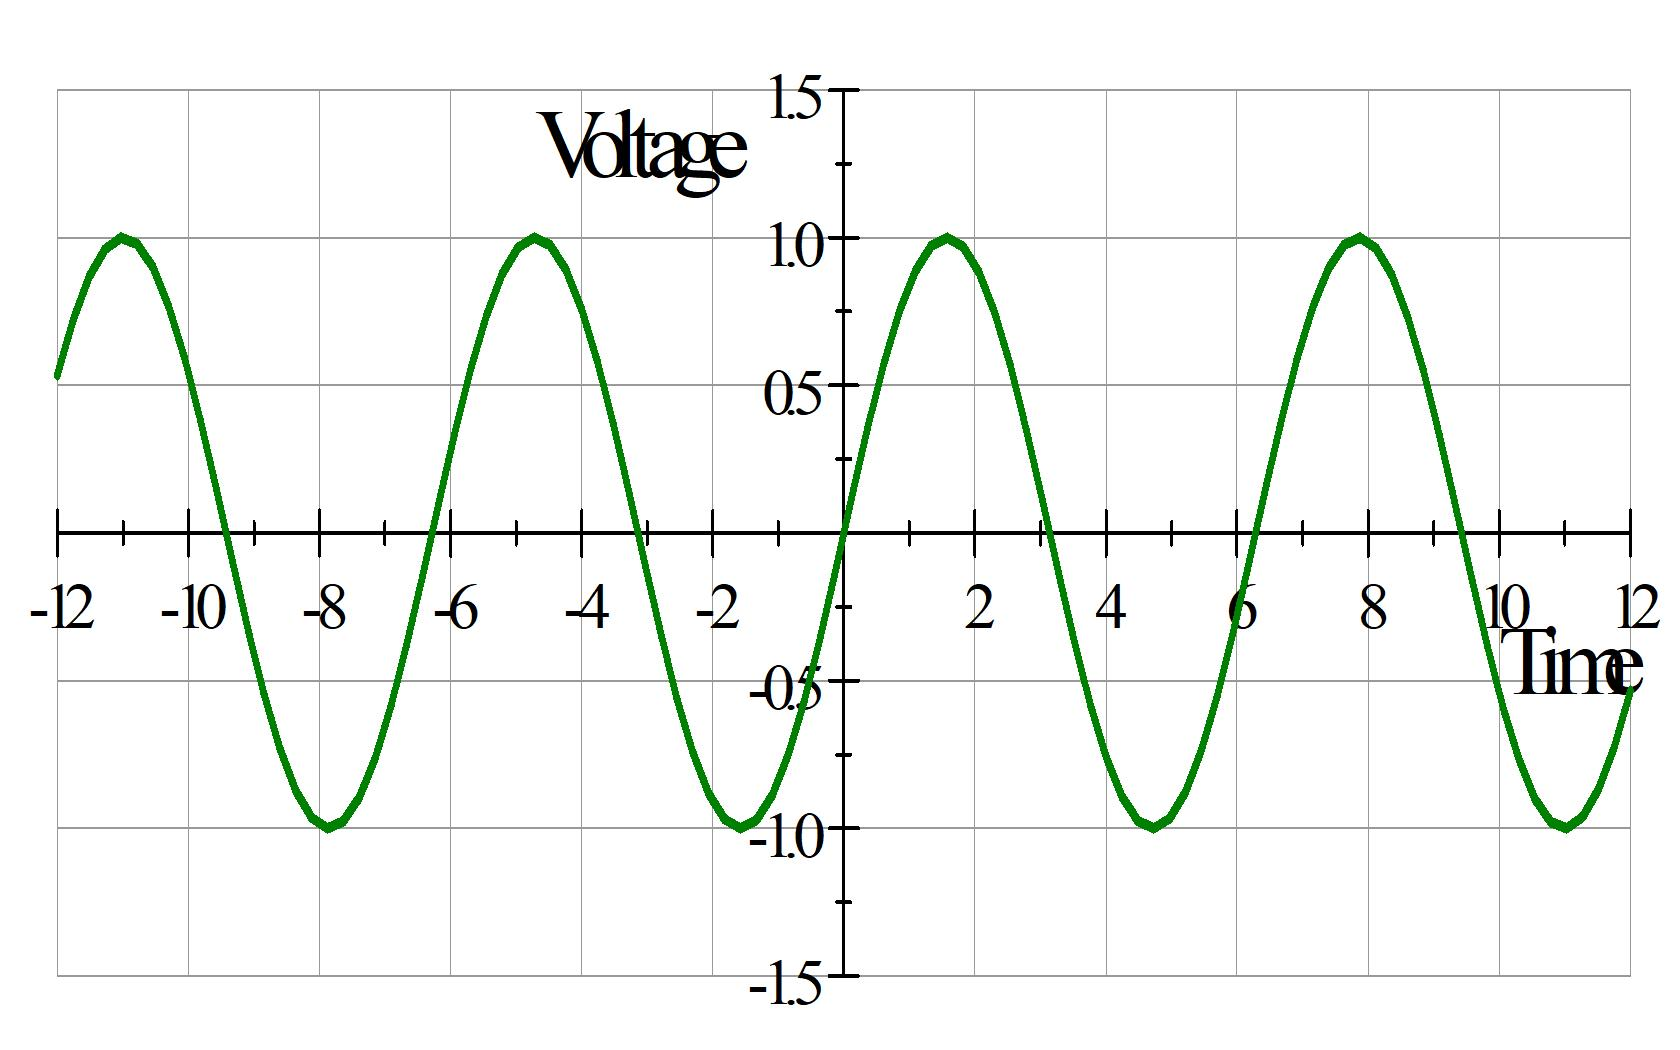
\includegraphics[width=4.4996in,height=1.8204in]{PH4CAX4H}
\end{figure}

The easiest way to fix this problem is to use, once again, use our voltage
divider. but this time we will fix each end at a different voltage. We will need one end at a positive voltage. The other can then go as negative as the first end is positive. Let's take a concrete example to show how this works.

Suppose we want to measure a voltage that could be as negative as $-5\unit{V}$ or as positive as $+5\unit{V}.$ We still need to map this to our $0$ to $5\unit{V}$ Arduino range. Consider the following voltage divider.
\begin{figure}[h!]
	\centering
	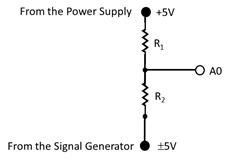
\includegraphics[width=1.9407in,height=1.3615in]{PH4CAX4I}
\end{figure}

Let's start by setting $R_{1}=R_{2}.$ Then any voltage at the junction between $R_{1}$ and $R_{2}$ should be midway between the voltages input on the top of $R_{1}$ and the Bottom of $R_{2}.$ We put in $+5\unit{V}$ from our power supply on the top. And suppose we hook $-5\unit{V}$ to the bottom (say, from our signal generator). We expect the voltage divider to divide the total voltage difference in half. We have $10\unit{V}$ range from $-5\unit{V}$ to $+5\unit{V}$. We expect the junction between $R_{1}$ and $R_{2}$ to be right in the middle of that range. So we expect to see $0\unit{V}$ on pin A0 when the signal generator outputs $-5\unit{V}.$ So far so good! Now suppose the signal generator gives us $+5\unit{V}.$ Half way between $+5\unit{V}$ and $+5\unit{V}$ is still $+5\unit{V}$. This is just what we want! Any voltage from the signal generator between $+5\unit{V}$ and $-5\unit{V}$ will end up between $0\unit{V}$ and $+5\unit{V}$ at input A0. For example, say we have $-2\unit{V}$ from the signal generator. The at $A0$ we will have a voltage half way between $+5\unit{V}$ and $-2\unit{V}.$ Pin A0 would have $1.5\unit{V}.$

We must be very careful to get this one wired right before we hook it to our Arduino. We also need to make sure our signal generator and power supply are plugged into grounded outlets so they have a common ground.

The oscilloscope, power supply, and signal generator are all grounded
through their grounded plugs. But our Arduino is not. We need to tie all the grounds of all our equipment together. So put a wire on the power supply negative output and wire it with an alligator clip to the grounded exterior of the signal generator TTL BNC connector. Then take another wire and connect it to the power supply negative output and wire this to a GND pin on the Arduino. This should ensure that all three devices have the same ground point (so we won't get a spark from one to another).

Before we hook this bit of electronics to our Arduino, we want to check it on one of our meters. But our multimeter is not the best choice. For this test, let's use the oscilloscope.

Our oscilloscopes have two channels where we can hook probes. Let's use one to measure the signal as it comes directly from the signal generator. Let's use the other to measure at the junction in between $R_{1}$ and $R_{2}$ right were we will connect pin A0. That should be our output. \begin{figure}[h!]
	\centering
	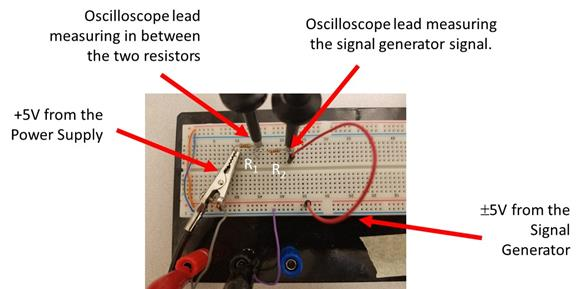
\includegraphics[width=4.9174in,height=2.4436in]{PH4CAX4J}
\end{figure}

What we see on the oscilloscope should look like this: 
\begin{figure}[h!]
	\centering
	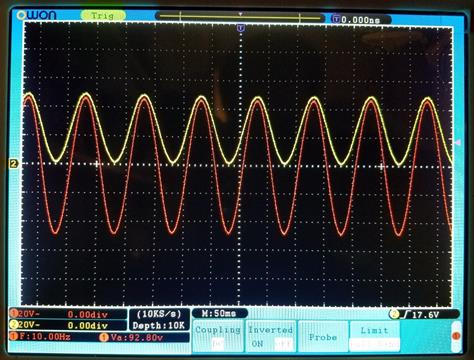
\includegraphics[width=3.9902in,height=3.0355in]{PH4CAX4K}
\end{figure}
The red trace is the signal from the signal generator. The yellow trace is from our voltage divider. Notice that our signal generator is giving us $-5\unit{V}$ to $+5\unit{V}$ and our output from the voltage divider is $0$ to $5\unit{V}$ just as we hoped.

Of course in our sketch, we have to do a little math to have our output at
the serial monitor be values from $-5\unit{V}$ to $+5\unit{V}.$ We mapped
this to $0$ to $5\unit{V}.$ That is a $10\unit{V}$ range into a $5\unit{V}$ range. So each volt measured pin A0 is really worth two volts that were input from the signal generator. But we are offset by $5\unit{V},$ so we need to multiply our $0$ to $5\unit{V}$ ADC units by 2 and subtract $5\unit{V}$
\begin{equation*}
	\Delta V_{measured}=2\Delta V_{ACD}-5\unit{V}
\end{equation*}



Notice that our minimum detectable voltage difference of $\Delta V_{ADC\min}=4.9\unit{mV}$ will map to 
\begin{eqnarray*}
	\delta V &=&2\left( 4.9\unit{mV}\right) \\
	         &=&9\,.8\unit{mV}
\end{eqnarray*}
We have a much higher uncertainty using this set up! So there was a cost to using this method of measuring both positive and negative voltages.

We can use the Oscilloscope stand-alone device to measure our voltages before we hook up our delicate Arduino. The Oscilloscope is designed to make this type of measurement. It likes periodic signals and it likes positive and negative voltages. It can handle fairly large voltages. It is nice because it plots the voltage vs. time graph. It has adjustment knobs to change the scale of the graph axes.

We can set up our circuit and clip the oscilloscope probe to either side of the capacitor. As we change the frequency of the signal generator the frequency of the voltage across the capacitor will change. As we get near the resonant frequency, the amplitude of the capacitor voltage will grow.
Right at the resonant frequency, $\Delta V_{C}$ will be largest. We will
need to measure this before using our Arduino to be sure the voltage won't
go over $5\unit{V}$. We need to keep it to less than $\pm 5\unit{V}$ at
resonance. If we keep changing the frequency the amplitude will go back
down. So when we see the amplitude grow, max out, and then diminish we know we have just passed resonance. This is just what we saw in last week's lab.

Once we have this working on our oscilloscope, we can try it on our Arduino. Of course we need a sketch for this. Here is a simple example.
\vspace{0.25in}
%%%%%%%%%%%%%%%%%%%%%%%%%%%%%%%%%%%%%%%%%%%%%%%%%%%%%%%%%%%%%%%%%%%%%%%%%%
\href{https://dtoliphant.github.io/PH250Manual/Code/RLCPart2_pm5Vsignal.ino}{Download here}
%%%%%%%%%%%%%%%%%%%%%%%%%%%%%%%%%%%%%%%%%%%%%%%%%%%%%%%%%%%%%%%%%%%%%%%%%%
\lstinputlisting[language=Arduino]{Code/RLCPart2_pm5Vsignal.ino}

So our new instrument takes in an alternating voltage, and displays it. We
will have to adjust the input voltage on the signal generator. When the
signal generator frequency is just right, the voltage we measure should
become large. By noting the resonant frequency we can check our model for
inductance.

\section{Sampling Theory, a complication}

Before we finish designing this experiment, we need to think about another
limitation of our Arduino devices. That is that they can only take up to $2000$ measurements in a second. We say they have a maximum sampling rate of $2000\unit{Hz}.$ To try to understand this, consider trying to measure a sine wave.

\begin{figure}[h!]
	\centering
	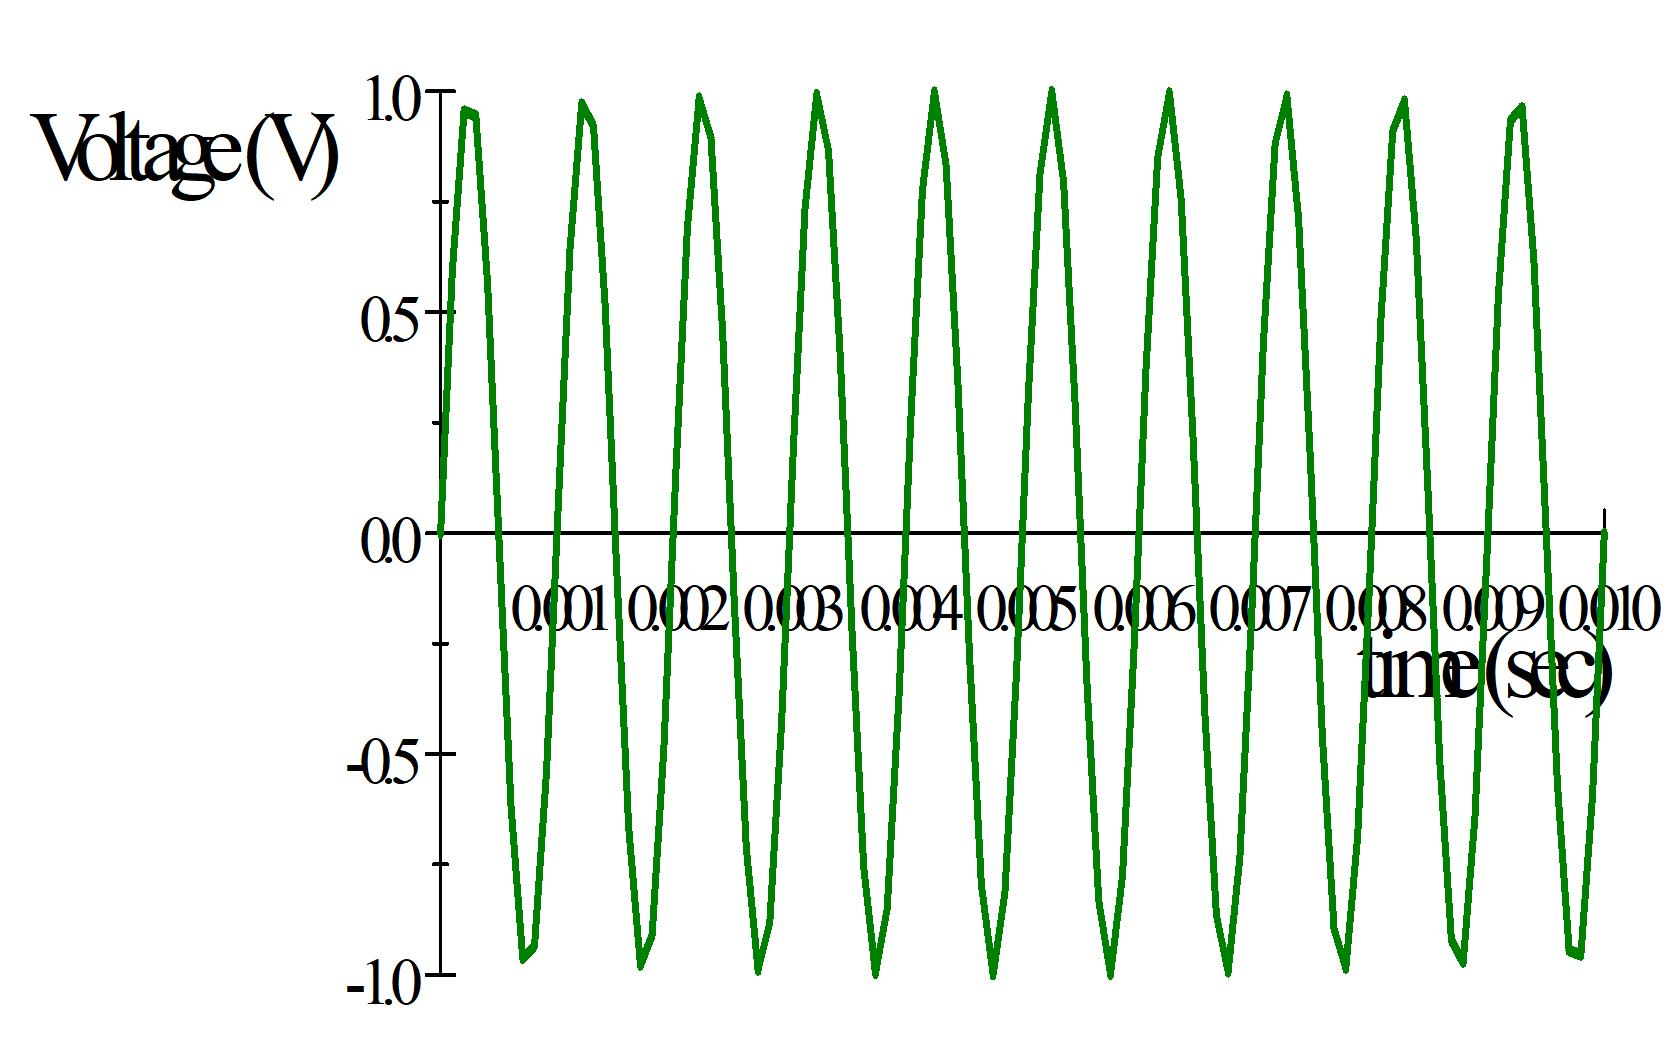
\includegraphics[width=4.4996in,height=1.7919in]{PH4CAX4L}
\end{figure}
There are an infinite number of points in a sign wave. That is, 
\begin{equation*}
	V\left( t\right) =\sin \left( \omega t\right)
\end{equation*}
for every $t$ at all. So ideally we would have an infinite number of $t$
values between $0$ and $1\unit{s}$ so that we would not miss any $V\left(
t\right) $ values. But our Arduino can't take an infinite number of values. It an only take up to $2000$ values a second. Suppose we have a signal frequency of $1000\unit{Hz}.$ That means there should be 
\begin{equation*}
	\frac{1}{1000\unit{Hz}}=0.001\,\unit{s}
\end{equation*}
in between peaks of our sine wave. And suppose we wish to measure this. We
can only measure at a rate of $2000\unit{Hz},$ so there will be 
\begin{equation*}
	\frac{1}{2000\unit{Hz}}=0.000\,5\unit{s}
\end{equation*}
between measurements. That would look like this

\begin{figure}[h!]
	\centering
	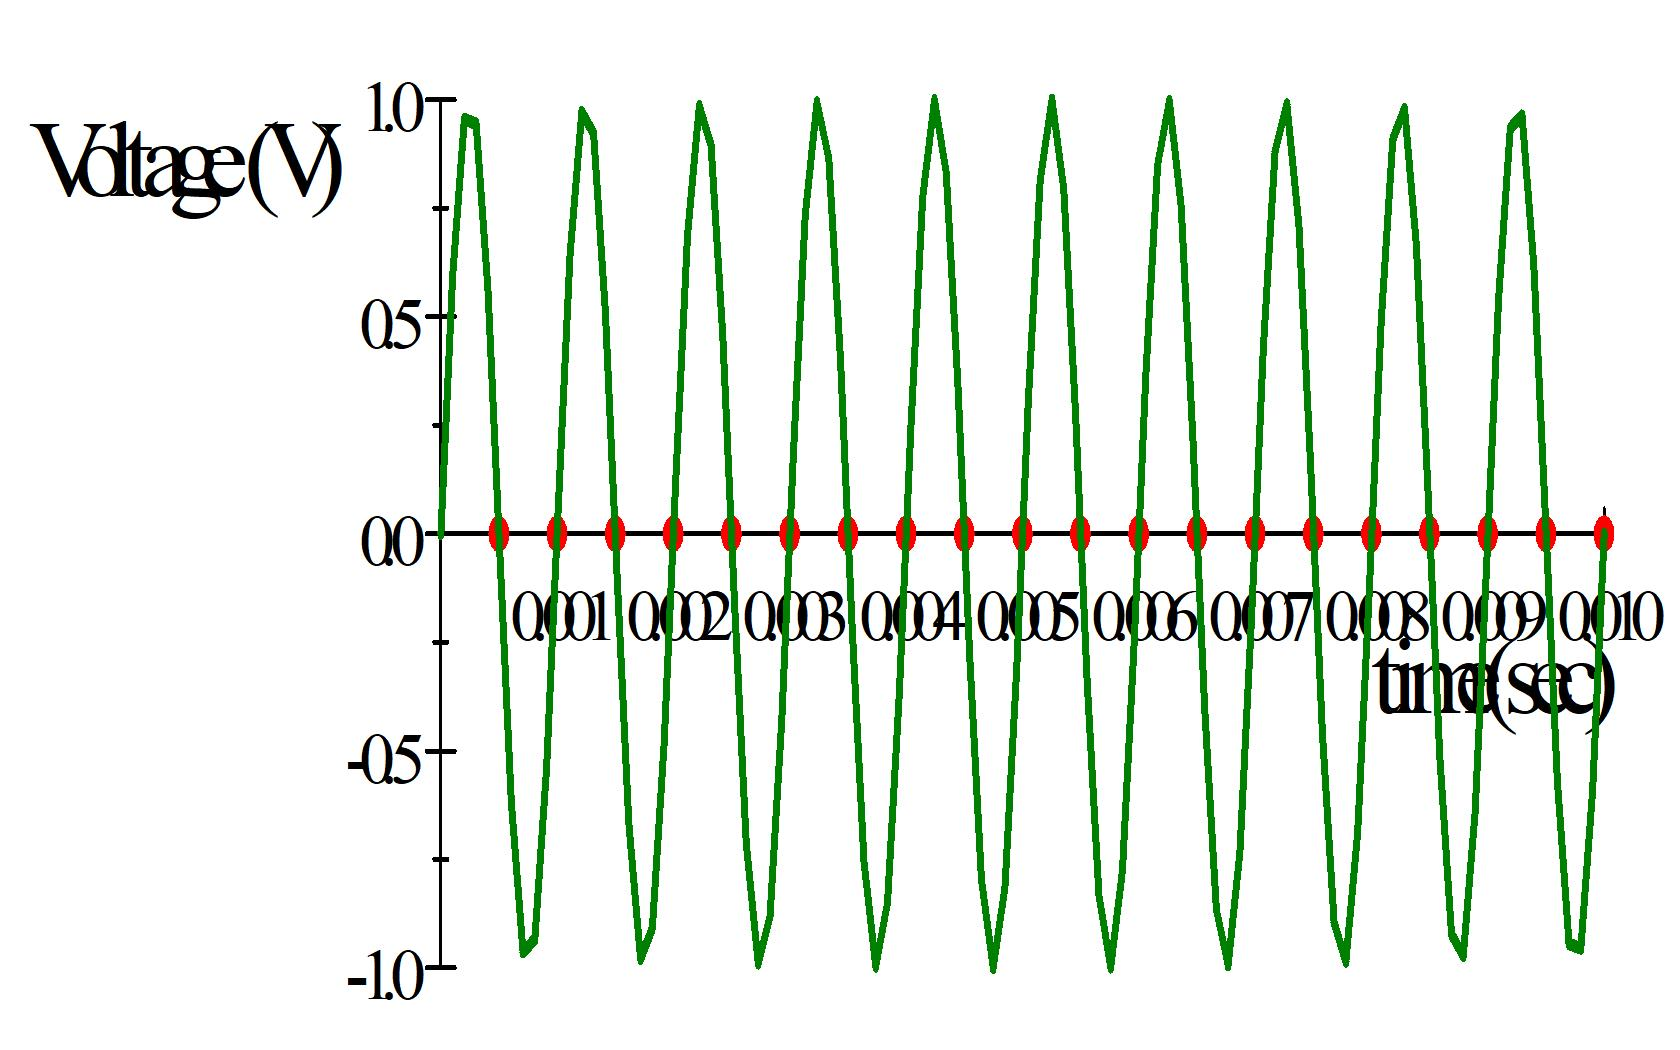
\includegraphics[width=4.4996in,height=1.6354in]{PH4CAX4M}
\end{figure}

where the red dots are the measurements. And look, we seem to have had back luck and we got all zeros!. This is no good! Because we are taking
measurements in sync with the sine wave, we get the false impression that we are measuring a constant voltage. Even if we offset the dots, it wouldn't help much.
\begin{figure}[h!]
	\centering
	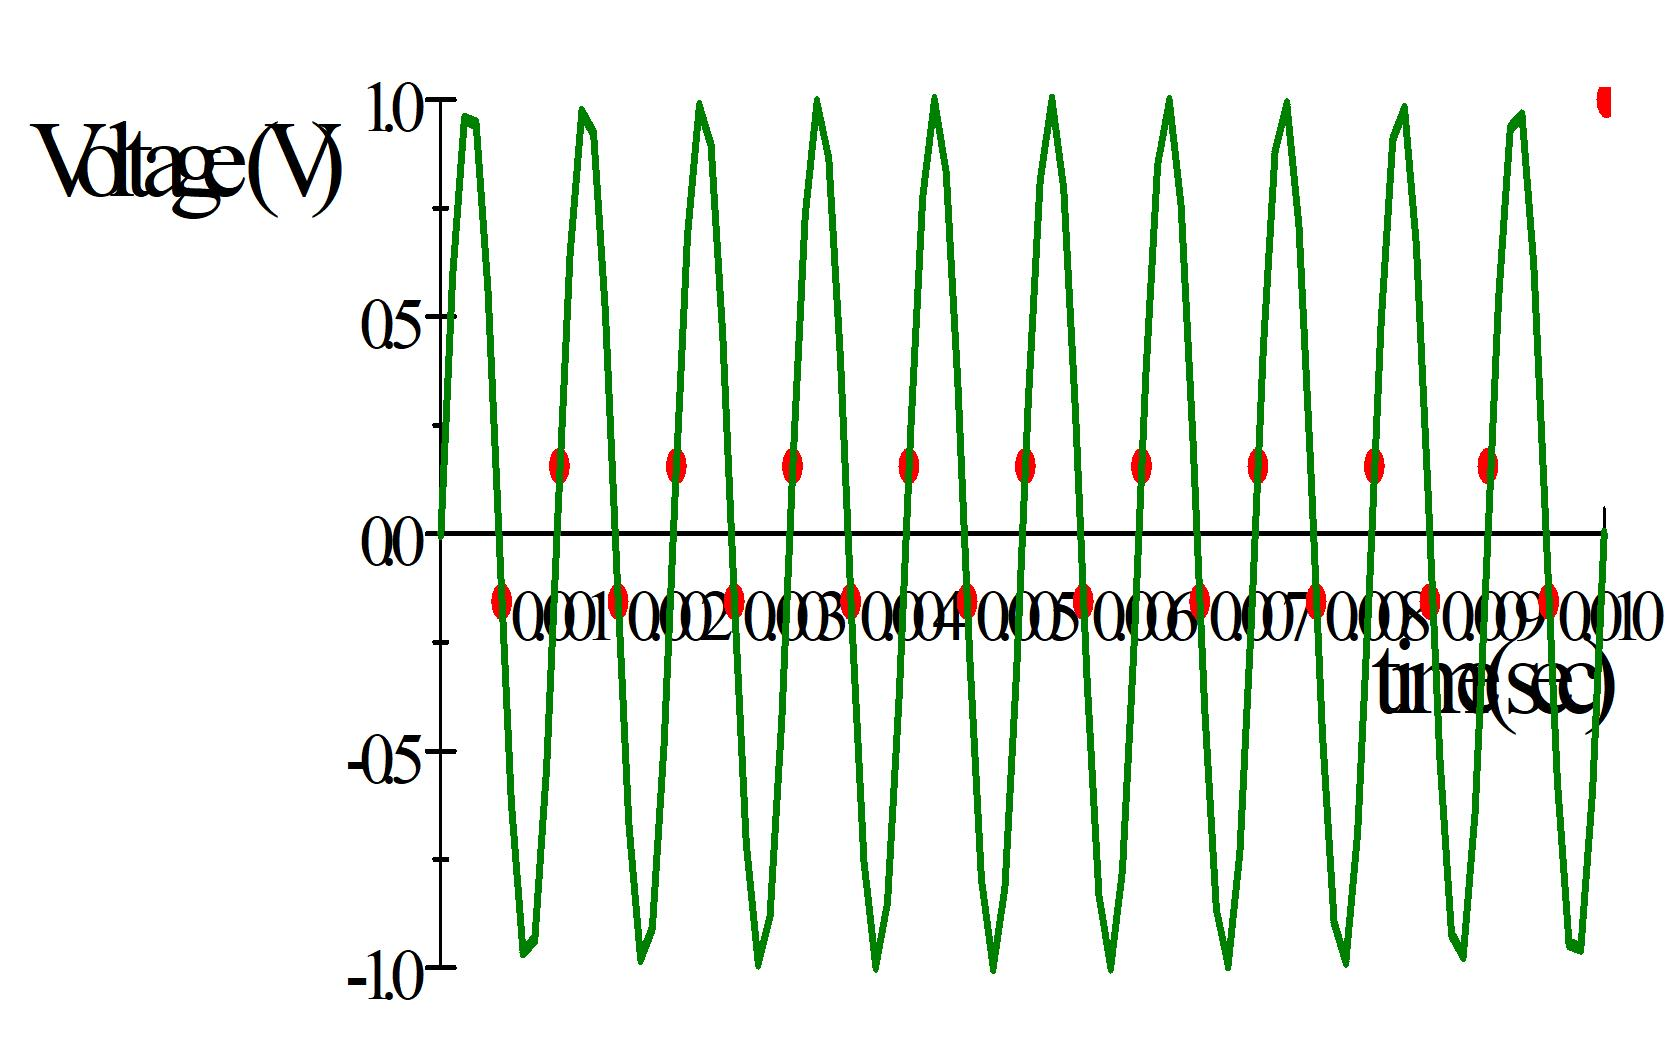
\includegraphics[width=4.4996in,height=1.6354in]{PH4CAX4N}
\end{figure}
Now we do see that we have some change in the voltage, but the measurements aren't representing the actual change. The solution to this problem is to lower our signal frequency so that we have more points per signal period. Say, we have a sine wave with a frequency of $250\unit{Hz}.$ Now our graph would look like this. 
\begin{figure}[h!]
	\centering
	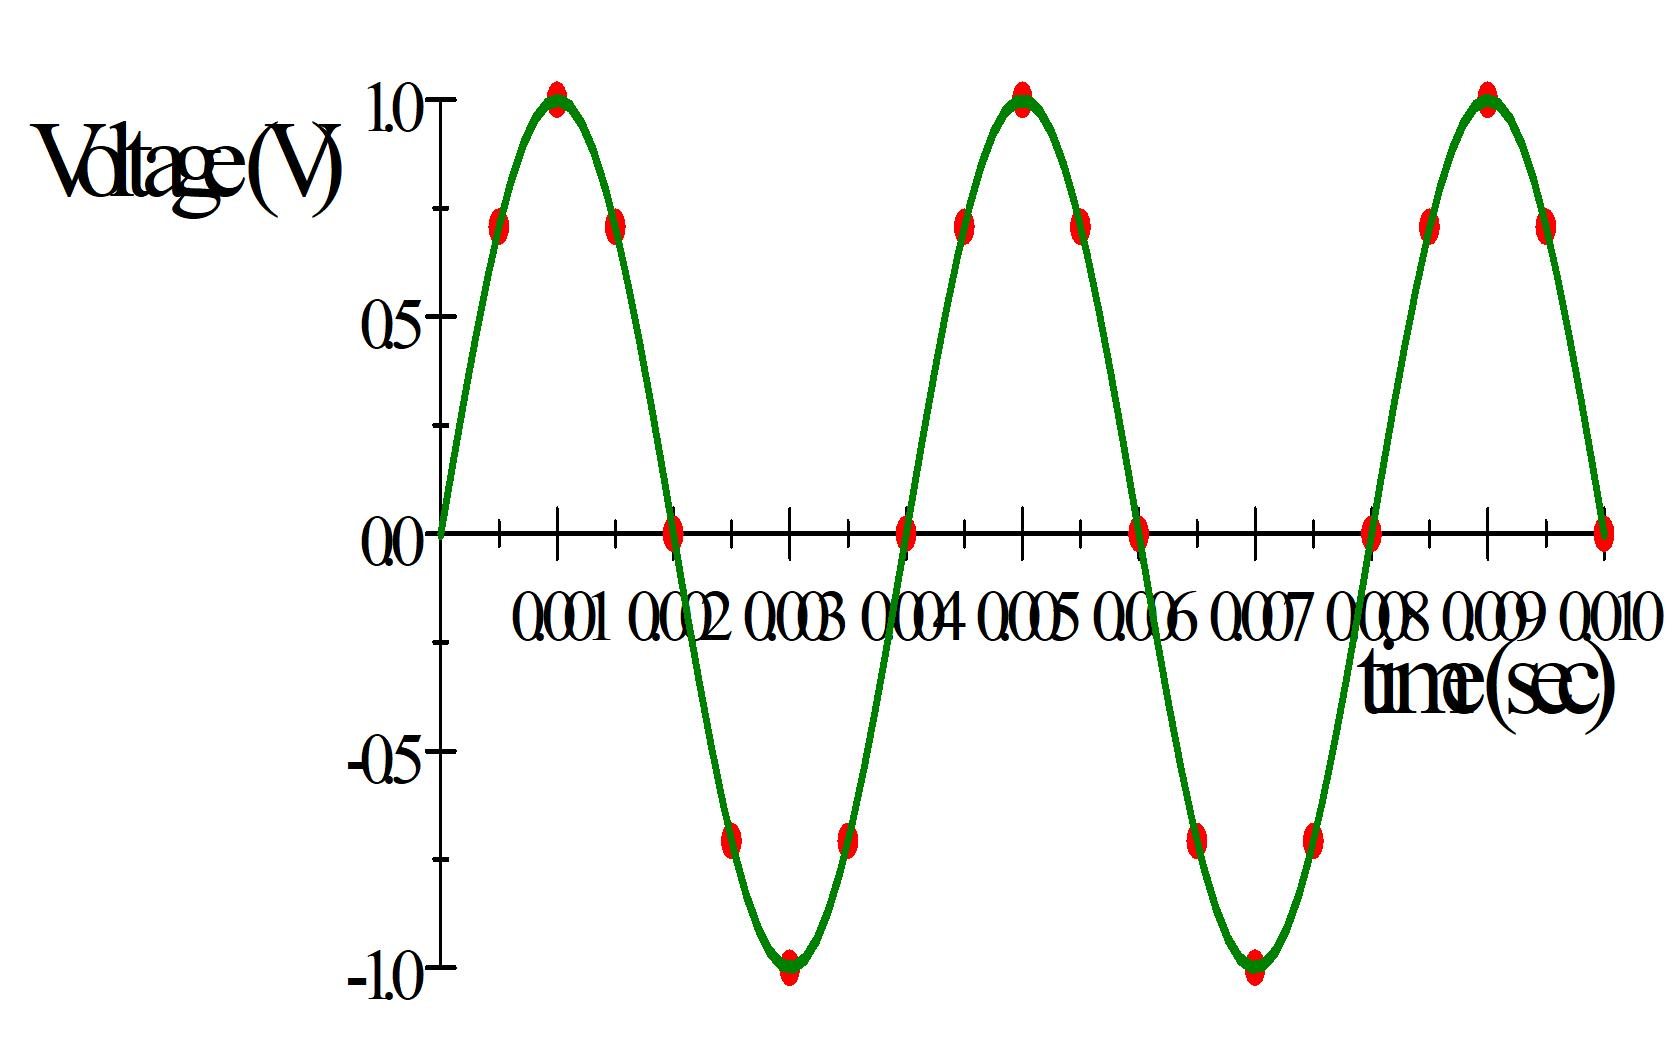
\includegraphics[width=4.4996in,height=1.6354in]{PH4CAX4O}
\end{figure}

Now if we just plotted the measurements, we could still tell it was a sine
wave.
\begin{figure}[h!]
	\centering
	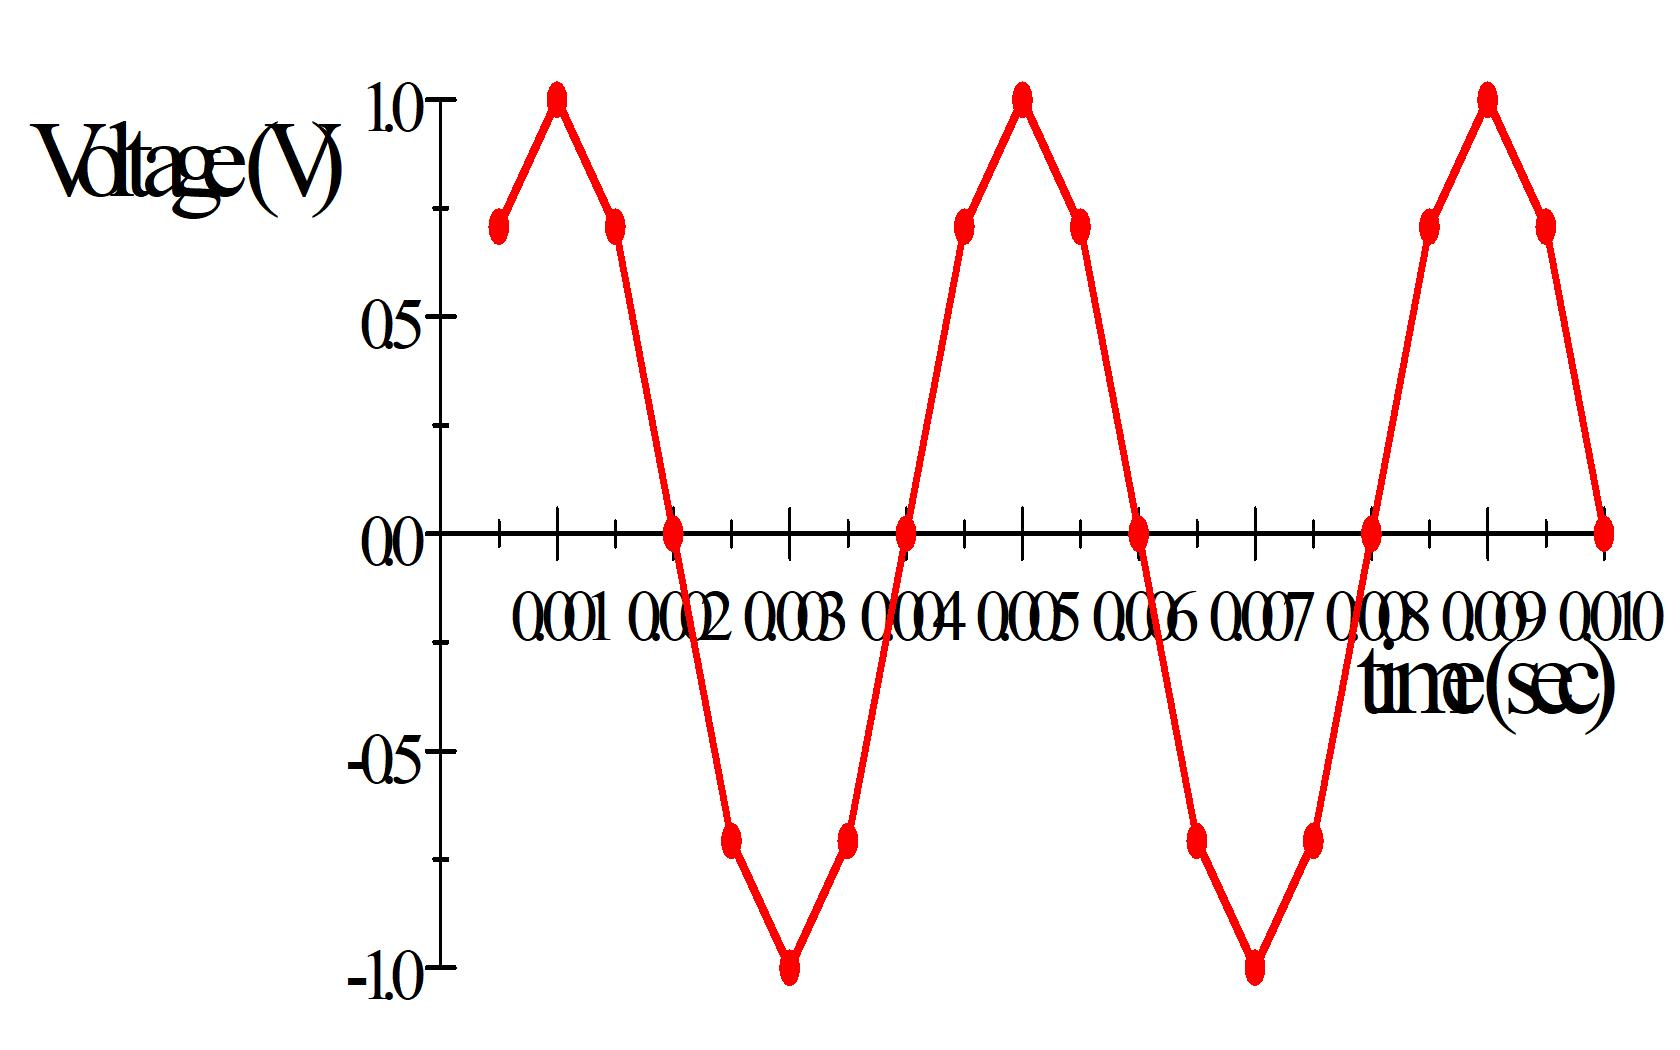
\includegraphics[width=4.4996in,height=1.6354in]{PH4CAX4P}
\end{figure}
Granted, it doesn't look great, but we wouldn't mistake it for a straight line. This problem of having to take measurements faster than our signal changes is called aliasing (because if you get it wrong, it looks like the wrong function came from the signal generator). We need to make sure our signal frequency is much lower (like ten times lower) than the frequency at which we can take measurements, or we will be fooled. Last lab, we had resonance frequencies that were around $20000\unit{Hz}.$ That is way too high for our Arduinos. We need to change capacitors so that our resonance frequency is more like $200\unit{Hz}$ or our measurements will be aliased. Suppose we use the following 
\begin{eqnarray*}
	\mathcal{E} &=&5\unit{V} \\
	          L &=&2.3\times 10^{-3}\unit{H} \\
	          R &=&10000\unit{\Omega} \\
  f_{resonance} &=&18.552\unit{kHz} \\
              C &=&32\times 10^{-6}\unit{F}
\end{eqnarray*}

We should get something like this for our resonance plot.

\begin{figure}[h!]
	\centering
	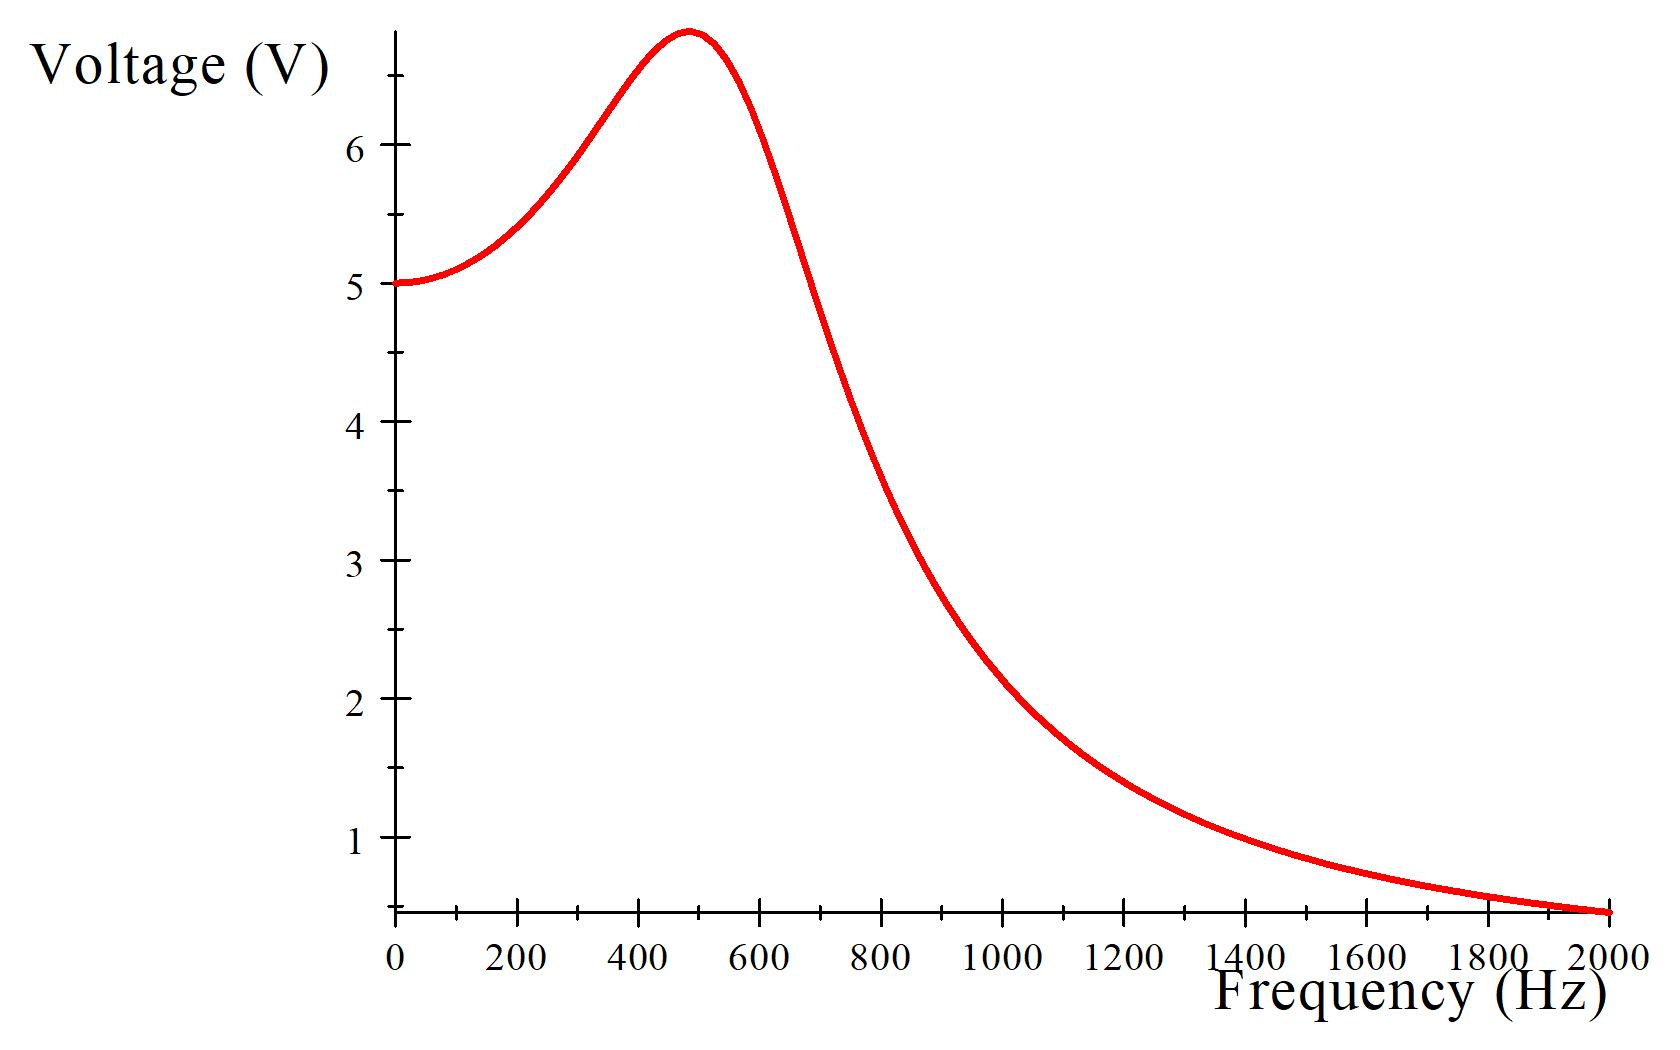
\includegraphics[width=4.4996in,height=3in]{PH4CAX4Q}
\end{figure}
And this we could reasonably detect. Our measurements might look somewhat ratty, but we should be able to see a sine wave and find when it is maximum.

\section{Lab Assignment}

\begin{enumerate}
	\item Estimate the inductance of your coil using equation \ref{Solenoid Inductance}. You may use your estimate from last week and any insight into that estimate that last week's measurements might have given you.

	\item Measuring the inductance using resonance with an Arduino based oscilloscope

	\begin{enumerate}
		\item Set up an $LRC$ circuit like we did last lab. Make sure your resistance is not too high using equation \ref{Criticall Damping Criteria}. Use one of our signal generators to produce as the source of variable emf. 
		\begin{figure}[h!]
			\centering
			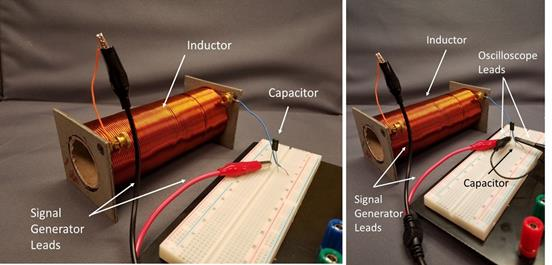
\includegraphics[width=4.6496in,height=2.2423in]{PH4CAX4R}
		\end{figure}

		\item Build the circuit described above to measure positive and negative voltages with our Arduios and the serial plotter.

		\item Predict the resonant frequency of your $LRC$ circuit using the large wire coils and something close to a $330\unit{nF}$ capacitor (Note, this is a different capacitance than last lab!). This is necessary because our Arduinos can only collect data $2000$ times a second. That limits the frequencies we can see.

		\item Set up an $LRC$ circuit with the new capacitor in it (really just keep the same circuit and swap out capacitors

		\item Test the circuit using the oscilloscope. Again you should see a nice sine wave, but now we need to be sure that the voltage is far less than our $5\unit{V}$ limit for our Arduino. We know the voltage is going to get bit at resonance. So we need to be careful! 
		\begin{figure}[h!]
			\centering
			
\includegraphics[width=2.8089in,height=1.4684in]{PH4CAX4S}
		\end{figure}

		\item Adjust your signal generator near your new natural frequency of oscillation. Note what happens to the amplitude as you tune the dial. This should be the same as what you saw on the Oscilloscope (I might suggest just leaving the oscilloscope connected).

		\item Once again, determine your actual resonant frequency, $f_{A}$.

		\item Once again, calculate your inductance based on $f_{A}$. Compare to your calculated value. If there is a difference, try to explain it.
	\end{enumerate}

	\item Now just for fun (time permitting), place a metal rod in your solenoid. Observe what happens to the amplitude. What happens to the resonant frequency? Discuss how metal detectors might work.

	\item Check with your professor to make sure everything is set to start your student designed project next week.
\end{enumerate}


\vfill
